\documentclass[tikz]{standalone}
\usepackage{amsmath,amssymb}
\usetikzlibrary{arrows.meta,positioning,calc}

\definecolor{deepblue}{RGB}{20,50,120}
\definecolor{lightblue}{RGB}{180,210,240}
\definecolor{goldaccent}{RGB}{200,170,50}
\definecolor{mydarkgray}{RGB}{60,60,60}
\definecolor{softgreen}{RGB}{60,150,80}
\definecolor{softred}{RGB}{200,60,60}

\begin{document}
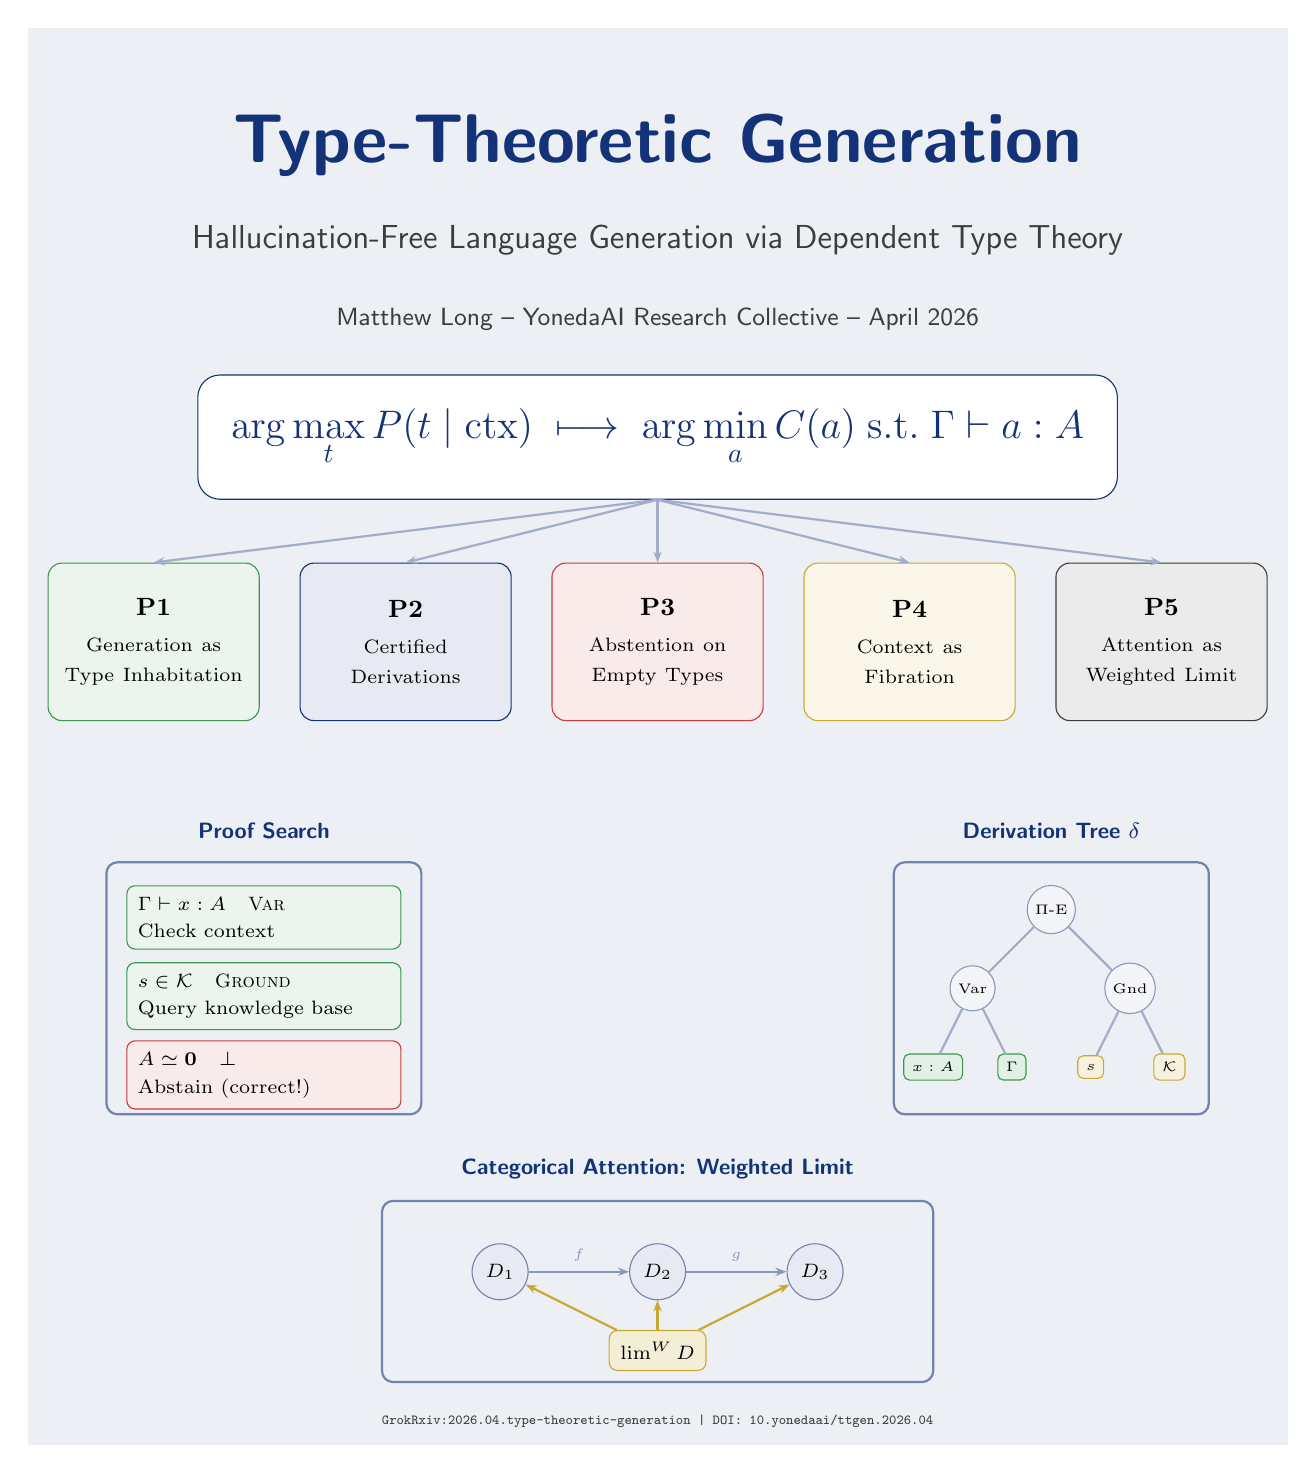
\begin{tikzpicture}[every node/.style={font=\sffamily}]

% Background
\fill[deepblue!8] (-8,-11) rectangle (8,7);

% Title
\node[font=\Huge\bfseries\sffamily, text=deepblue, text width=14cm, align=center]
  at (0,5.5) {Type-Theoretic Generation};
\node[font=\large\sffamily, text=mydarkgray, text width=14cm, align=center]
  at (0,4.3) {Hallucination-Free Language Generation via Dependent Type Theory};

% Author
\node[font=\small\sffamily, text=mydarkgray] at (0,3.3)
  {Matthew Long -- YonedaAI Research Collective -- April 2026};

% Central equation
\node[draw=deepblue, fill=white, rounded corners=8pt, inner sep=12pt,
      font=\Large, text=deepblue] (eq) at (0,1.8)
  {$\displaystyle\arg\max_t P(t \mid \mathrm{ctx}) \;\longmapsto\;
    \arg\min_a C(a) \;\text{s.t.}\; \Gamma \vdash a : A$};

% Five principles
\node[draw=softgreen, fill=softgreen!10, rounded corners=5pt,
      minimum width=2.6cm, minimum height=2.0cm,
      text width=2.4cm, align=center, inner sep=4pt,
      font=\small] (p1) at (-6.4,-0.8)
  {\textbf{P1}\\[2pt]{\scriptsize Generation as Type Inhabitation}};

\node[draw=deepblue, fill=deepblue!10, rounded corners=5pt,
      minimum width=2.6cm, minimum height=2.0cm,
      text width=2.4cm, align=center, inner sep=4pt,
      font=\small] (p2) at (-3.2,-0.8)
  {\textbf{P2}\\[2pt]{\scriptsize Certified Derivations}};

\node[draw=softred, fill=softred!10, rounded corners=5pt,
      minimum width=2.6cm, minimum height=2.0cm,
      text width=2.4cm, align=center, inner sep=4pt,
      font=\small] (p3) at (0,-0.8)
  {\textbf{P3}\\[2pt]{\scriptsize Abstention on Empty Types}};

\node[draw=goldaccent, fill=goldaccent!10, rounded corners=5pt,
      minimum width=2.6cm, minimum height=2.0cm,
      text width=2.4cm, align=center, inner sep=4pt,
      font=\small] (p4) at (3.2,-0.8)
  {\textbf{P4}\\[2pt]{\scriptsize Context as Fibration}};

\node[draw=mydarkgray, fill=mydarkgray!10, rounded corners=5pt,
      minimum width=2.6cm, minimum height=2.0cm,
      text width=2.4cm, align=center, inner sep=4pt,
      font=\small] (p5) at (6.4,-0.8)
  {\textbf{P5}\\[2pt]{\scriptsize Attention as Weighted Limit}};

% Arrows
\draw[-{Stealth[length=4pt]}, deepblue!40, thick] (eq.south) -- (p1.north);
\draw[-{Stealth[length=4pt]}, deepblue!40, thick] (eq.south) -- (p2.north);
\draw[-{Stealth[length=4pt]}, deepblue!40, thick] (eq.south) -- (p3.north);
\draw[-{Stealth[length=4pt]}, deepblue!40, thick] (eq.south) -- (p4.north);
\draw[-{Stealth[length=4pt]}, deepblue!40, thick] (eq.south) -- (p5.north);

% Proof search box
\node[font=\footnotesize\sffamily\bfseries, text=deepblue] at (-5,-3.2) {Proof Search};
\draw[thick, deepblue!60, rounded corners=4pt] (-7,-3.6) rectangle (-3,-6.8);
\node[draw=softgreen, fill=softgreen!10, rounded corners=3pt,
      font=\scriptsize, inner sep=4pt, text width=3.2cm, align=left]
  at (-5,-4.3) {$\Gamma \vdash x : A$\quad\textsc{Var}\\[2pt]Check context};
\node[draw=softgreen, fill=softgreen!10, rounded corners=3pt,
      font=\scriptsize, inner sep=4pt, text width=3.2cm, align=left]
  at (-5,-5.3) {$s \in \mathcal{K}$\quad\textsc{Ground}\\[2pt]Query knowledge base};
\node[draw=softred, fill=softred!10, rounded corners=3pt,
      font=\scriptsize, inner sep=4pt, text width=3.2cm, align=left]
  at (-5,-6.3) {$A \simeq \mathbf{0}$\quad$\bot$\\[2pt]Abstain (correct!)};

% Derivation tree box
\node[font=\footnotesize\sffamily\bfseries, text=deepblue] at (5,-3.2) {Derivation Tree $\delta$};
\draw[thick, deepblue!60, rounded corners=4pt] (3,-3.6) rectangle (7,-6.8);

\node[draw=deepblue!50, fill=deepblue!5, circle, inner sep=2pt,
      font=\tiny] (root) at (5,-4.2) {$\Pi$-E};
\node[draw=deepblue!50, fill=deepblue!5, circle, inner sep=2pt,
      font=\tiny] (l1) at (4,-5.2) {Var};
\node[draw=deepblue!50, fill=deepblue!5, circle, inner sep=2pt,
      font=\tiny] (r1) at (6,-5.2) {Gnd};
\node[draw=softgreen, fill=softgreen!15, rounded corners=2pt,
      font=\tiny, inner sep=3pt] (leaf1) at (3.5,-6.2) {$x:A$};
\node[draw=softgreen, fill=softgreen!15, rounded corners=2pt,
      font=\tiny, inner sep=3pt] (leaf2) at (4.5,-6.2) {$\Gamma$};
\node[draw=goldaccent, fill=goldaccent!15, rounded corners=2pt,
      font=\tiny, inner sep=3pt] (leaf3) at (5.5,-6.2) {$s$};
\node[draw=goldaccent, fill=goldaccent!15, rounded corners=2pt,
      font=\tiny, inner sep=3pt] (leaf4) at (6.5,-6.2) {$\mathcal{K}$};

\draw[thick, deepblue!40] (root) -- (l1);
\draw[thick, deepblue!40] (root) -- (r1);
\draw[thick, deepblue!40] (l1) -- (leaf1);
\draw[thick, deepblue!40] (l1) -- (leaf2);
\draw[thick, deepblue!40] (r1) -- (leaf3);
\draw[thick, deepblue!40] (r1) -- (leaf4);

% Categorical attention
\node[font=\footnotesize\sffamily\bfseries, text=deepblue] at (0,-7.5)
  {Categorical Attention: Weighted Limit};
\draw[thick, deepblue!60, rounded corners=4pt] (-3.5,-7.9) rectangle (3.5,-10.2);

\node[draw=deepblue!60, fill=deepblue!10, circle, inner sep=3pt,
      font=\scriptsize] (d1) at (-2,-8.8) {$D_1$};
\node[draw=deepblue!60, fill=deepblue!10, circle, inner sep=3pt,
      font=\scriptsize] (d2) at (0,-8.8) {$D_2$};
\node[draw=deepblue!60, fill=deepblue!10, circle, inner sep=3pt,
      font=\scriptsize] (d3) at (2,-8.8) {$D_3$};
\node[draw=goldaccent, fill=goldaccent!20, rounded corners=3pt,
      inner sep=4pt, font=\scriptsize\bfseries] (lim) at (0,-9.8) {$\lim^W D$};

\draw[-{Stealth[length=4pt]}, deepblue!50, thick] (d1) -- (d2)
  node[midway, above, font=\tiny] {$f$};
\draw[-{Stealth[length=4pt]}, deepblue!50, thick] (d2) -- (d3)
  node[midway, above, font=\tiny] {$g$};
\draw[-{Stealth[length=4pt]}, goldaccent, thick] (lim) -- (d1);
\draw[-{Stealth[length=4pt]}, goldaccent, thick] (lim) -- (d2);
\draw[-{Stealth[length=4pt]}, goldaccent, thick] (lim) -- (d3);

% DOI
\node[font=\tiny\ttfamily, text=mydarkgray] at (0,-10.7)
  {GrokRxiv:2026.04.type-theoretic-generation | DOI: 10.yonedaai/ttgen.2026.04};

\end{tikzpicture}
\end{document}
